\documentclass[]{article}
\usepackage{lmodern}
\usepackage{amssymb,amsmath}
\usepackage{ifxetex,ifluatex}
\usepackage{fixltx2e} % provides \textsubscript
\ifnum 0\ifxetex 1\fi\ifluatex 1\fi=0 % if pdftex
  \usepackage[T1]{fontenc}
  \usepackage[utf8]{inputenc}
\else % if luatex or xelatex
  \ifxetex
    \usepackage{mathspec}
  \else
    \usepackage{fontspec}
  \fi
  \defaultfontfeatures{Ligatures=TeX,Scale=MatchLowercase}
\fi
% use upquote if available, for straight quotes in verbatim environments
\IfFileExists{upquote.sty}{\usepackage{upquote}}{}
% use microtype if available
\IfFileExists{microtype.sty}{%
\usepackage{microtype}
\UseMicrotypeSet[protrusion]{basicmath} % disable protrusion for tt fonts
}{}
\usepackage[margin=1in]{geometry}
\usepackage{hyperref}
\hypersetup{unicode=true,
            pdfborder={0 0 0},
            breaklinks=true}
\urlstyle{same}  % don't use monospace font for urls
\usepackage{color}
\usepackage{fancyvrb}
\newcommand{\VerbBar}{|}
\newcommand{\VERB}{\Verb[commandchars=\\\{\}]}
\DefineVerbatimEnvironment{Highlighting}{Verbatim}{commandchars=\\\{\}}
% Add ',fontsize=\small' for more characters per line
\usepackage{framed}
\definecolor{shadecolor}{RGB}{248,248,248}
\newenvironment{Shaded}{\begin{snugshade}}{\end{snugshade}}
\newcommand{\AlertTok}[1]{\textcolor[rgb]{0.94,0.16,0.16}{#1}}
\newcommand{\AnnotationTok}[1]{\textcolor[rgb]{0.56,0.35,0.01}{\textbf{\textit{#1}}}}
\newcommand{\AttributeTok}[1]{\textcolor[rgb]{0.77,0.63,0.00}{#1}}
\newcommand{\BaseNTok}[1]{\textcolor[rgb]{0.00,0.00,0.81}{#1}}
\newcommand{\BuiltInTok}[1]{#1}
\newcommand{\CharTok}[1]{\textcolor[rgb]{0.31,0.60,0.02}{#1}}
\newcommand{\CommentTok}[1]{\textcolor[rgb]{0.56,0.35,0.01}{\textit{#1}}}
\newcommand{\CommentVarTok}[1]{\textcolor[rgb]{0.56,0.35,0.01}{\textbf{\textit{#1}}}}
\newcommand{\ConstantTok}[1]{\textcolor[rgb]{0.00,0.00,0.00}{#1}}
\newcommand{\ControlFlowTok}[1]{\textcolor[rgb]{0.13,0.29,0.53}{\textbf{#1}}}
\newcommand{\DataTypeTok}[1]{\textcolor[rgb]{0.13,0.29,0.53}{#1}}
\newcommand{\DecValTok}[1]{\textcolor[rgb]{0.00,0.00,0.81}{#1}}
\newcommand{\DocumentationTok}[1]{\textcolor[rgb]{0.56,0.35,0.01}{\textbf{\textit{#1}}}}
\newcommand{\ErrorTok}[1]{\textcolor[rgb]{0.64,0.00,0.00}{\textbf{#1}}}
\newcommand{\ExtensionTok}[1]{#1}
\newcommand{\FloatTok}[1]{\textcolor[rgb]{0.00,0.00,0.81}{#1}}
\newcommand{\FunctionTok}[1]{\textcolor[rgb]{0.00,0.00,0.00}{#1}}
\newcommand{\ImportTok}[1]{#1}
\newcommand{\InformationTok}[1]{\textcolor[rgb]{0.56,0.35,0.01}{\textbf{\textit{#1}}}}
\newcommand{\KeywordTok}[1]{\textcolor[rgb]{0.13,0.29,0.53}{\textbf{#1}}}
\newcommand{\NormalTok}[1]{#1}
\newcommand{\OperatorTok}[1]{\textcolor[rgb]{0.81,0.36,0.00}{\textbf{#1}}}
\newcommand{\OtherTok}[1]{\textcolor[rgb]{0.56,0.35,0.01}{#1}}
\newcommand{\PreprocessorTok}[1]{\textcolor[rgb]{0.56,0.35,0.01}{\textit{#1}}}
\newcommand{\RegionMarkerTok}[1]{#1}
\newcommand{\SpecialCharTok}[1]{\textcolor[rgb]{0.00,0.00,0.00}{#1}}
\newcommand{\SpecialStringTok}[1]{\textcolor[rgb]{0.31,0.60,0.02}{#1}}
\newcommand{\StringTok}[1]{\textcolor[rgb]{0.31,0.60,0.02}{#1}}
\newcommand{\VariableTok}[1]{\textcolor[rgb]{0.00,0.00,0.00}{#1}}
\newcommand{\VerbatimStringTok}[1]{\textcolor[rgb]{0.31,0.60,0.02}{#1}}
\newcommand{\WarningTok}[1]{\textcolor[rgb]{0.56,0.35,0.01}{\textbf{\textit{#1}}}}
\usepackage{graphicx,grffile}
\makeatletter
\def\maxwidth{\ifdim\Gin@nat@width>\linewidth\linewidth\else\Gin@nat@width\fi}
\def\maxheight{\ifdim\Gin@nat@height>\textheight\textheight\else\Gin@nat@height\fi}
\makeatother
% Scale images if necessary, so that they will not overflow the page
% margins by default, and it is still possible to overwrite the defaults
% using explicit options in \includegraphics[width, height, ...]{}
\setkeys{Gin}{width=\maxwidth,height=\maxheight,keepaspectratio}
\IfFileExists{parskip.sty}{%
\usepackage{parskip}
}{% else
\setlength{\parindent}{0pt}
\setlength{\parskip}{6pt plus 2pt minus 1pt}
}
\setlength{\emergencystretch}{3em}  % prevent overfull lines
\providecommand{\tightlist}{%
  \setlength{\itemsep}{0pt}\setlength{\parskip}{0pt}}
\setcounter{secnumdepth}{0}
% Redefines (sub)paragraphs to behave more like sections
\ifx\paragraph\undefined\else
\let\oldparagraph\paragraph
\renewcommand{\paragraph}[1]{\oldparagraph{#1}\mbox{}}
\fi
\ifx\subparagraph\undefined\else
\let\oldsubparagraph\subparagraph
\renewcommand{\subparagraph}[1]{\oldsubparagraph{#1}\mbox{}}
\fi

%%% Use protect on footnotes to avoid problems with footnotes in titles
\let\rmarkdownfootnote\footnote%
\def\footnote{\protect\rmarkdownfootnote}

%%% Change title format to be more compact
\usepackage{titling}

% Create subtitle command for use in maketitle
\providecommand{\subtitle}[1]{
  \posttitle{
    \begin{center}\large#1\end{center}
    }
}

\setlength{\droptitle}{-2em}

  \title{}
    \pretitle{\vspace{\droptitle}}
  \posttitle{}
    \author{}
    \preauthor{}\postauthor{}
    \date{}
    \predate{}\postdate{}
  

\begin{document}

\hypertarget{paneldata}{%
\section{Панельные данные}\label{paneldata}}

Загрузим необходимые библиотеки.

\begin{Shaded}
\begin{Highlighting}[]
\KeywordTok{library}\NormalTok{(foreign) }\CommentTok{#Вспомогательная библиотека для подгрузки данных}
\KeywordTok{library}\NormalTok{(plm) }\CommentTok{#Пакет для работы с панельными данными}
\KeywordTok{library}\NormalTok{(lmtest) }\CommentTok{#Пакет для оценки регрессий и ковариационных матриц параметров}
\KeywordTok{library}\NormalTok{(skimr) }\CommentTok{#Для красивого summary}
\KeywordTok{library}\NormalTok{(car) }\CommentTok{#Для некоторых графиков}
\KeywordTok{library}\NormalTok{(gplots) }\CommentTok{#Для графигов гетерогенности}
\KeywordTok{library}\NormalTok{(rio)}
\KeywordTok{library}\NormalTok{(tidyverse)}
\KeywordTok{library}\NormalTok{(car)}
\end{Highlighting}
\end{Shaded}

Загрузим данные, и преобразуем нужные переменные в факторные.В данном
разделе все визуализации будут построены на подмножестве данных из шести
наблюдений. Это позволит сделать их более читаемыми в формате книги. Все
модели будут оценены на всём массиве данных.

\begin{Shaded}
\begin{Highlighting}[]
\NormalTok{panel =}\StringTok{ }\KeywordTok{read_csv}\NormalTok{(}\StringTok{'lwage_panel_small.csv'}\NormalTok{)}
\NormalTok{panel}\OperatorTok{$}\NormalTok{black =}\StringTok{ }\KeywordTok{factor}\NormalTok{(panel}\OperatorTok{$}\NormalTok{black)}
\NormalTok{panel}\OperatorTok{$}\NormalTok{id =}\StringTok{ }\KeywordTok{factor}\NormalTok{(panel}\OperatorTok{$}\NormalTok{id)}
\end{Highlighting}
\end{Shaded}

Изобразим наши панельные данные на диаграмме рассеяния. Дополнимельно
установим параметр сглаживания, чтобы получить кривые временных рядов.

\begin{Shaded}
\begin{Highlighting}[]
\KeywordTok{scatterplot}\NormalTok{(lwage }\OperatorTok{~}\StringTok{ }\NormalTok{year}\OperatorTok{|}\NormalTok{id, }\DataTypeTok{boxplots=}\NormalTok{F, }\DataTypeTok{smooth=}\OtherTok{TRUE}\NormalTok{, }\DataTypeTok{regLine=}\OtherTok{FALSE}\NormalTok{, }\DataTypeTok{data=}\NormalTok{panel)}
\end{Highlighting}
\end{Shaded}

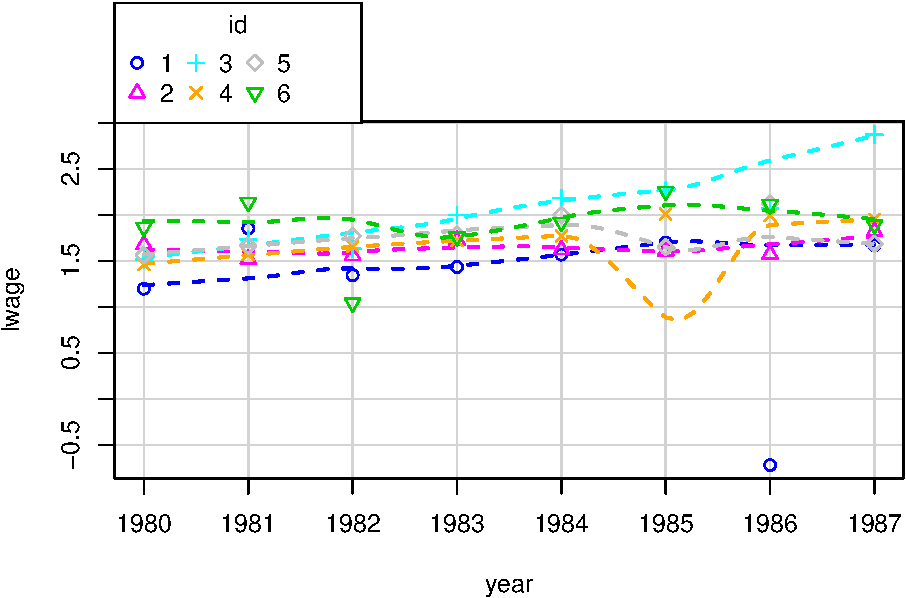
\includegraphics{09-paneldata_files/figure-latex/scatterplot chunk-1.pdf}

Для получения графиков на различных плитках можно использовать coplot.

\begin{Shaded}
\begin{Highlighting}[]
\KeywordTok{coplot}\NormalTok{(lwage }\OperatorTok{~}\StringTok{ }\NormalTok{year}\OperatorTok{|}\NormalTok{id, }\DataTypeTok{type =} \StringTok{'b'}\NormalTok{, }\DataTypeTok{data =}\NormalTok{ panel)}
\end{Highlighting}
\end{Shaded}

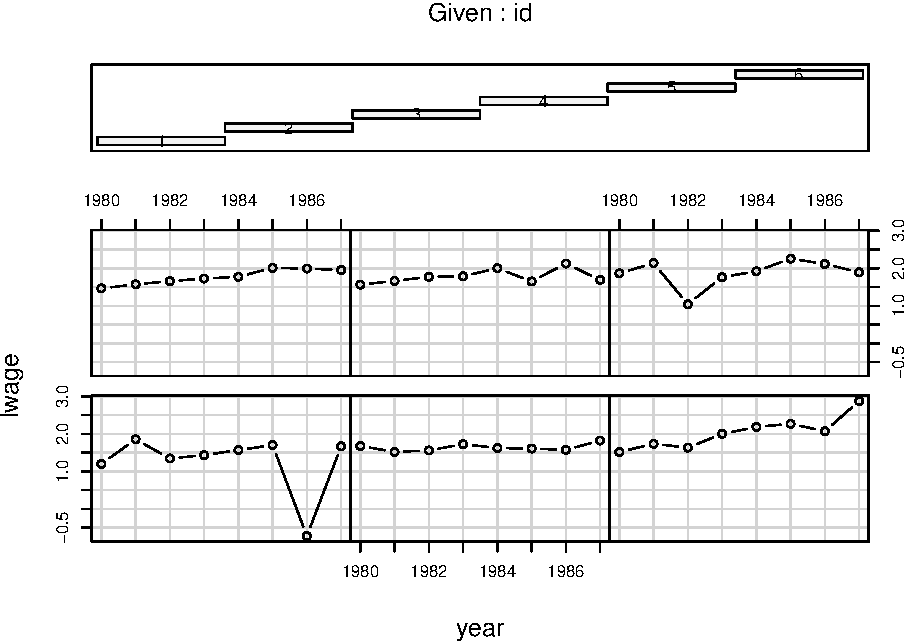
\includegraphics{09-paneldata_files/figure-latex/1 coplot chunk-1.pdf}

Сгруппировать можно по разным признакам. Например, в зависимости от расы
индивидов.

\begin{Shaded}
\begin{Highlighting}[]
\NormalTok{panel}\OperatorTok{$}\NormalTok{year =}\StringTok{ }\KeywordTok{factor}\NormalTok{(panel}\OperatorTok{$}\NormalTok{year)}
\KeywordTok{coplot}\NormalTok{(lwage }\OperatorTok{~}\StringTok{ }\NormalTok{year}\OperatorTok{|}\NormalTok{black, }\DataTypeTok{type=}\StringTok{"l"}\NormalTok{, }\DataTypeTok{data=}\NormalTok{panel, }\DataTypeTok{panel =} \ControlFlowTok{function}\NormalTok{(x, y, ...) }\KeywordTok{panel.smooth}\NormalTok{(x, y, }\DataTypeTok{span =} \FloatTok{0.3}\NormalTok{, ...), }\DataTypeTok{pch =} \DecValTok{16}\NormalTok{, }\DataTypeTok{show.given =}\NormalTok{ F, }\DataTypeTok{xlab =} \StringTok{"Mean dependence lwage of year for white and black people"}\NormalTok{)}
\end{Highlighting}
\end{Shaded}

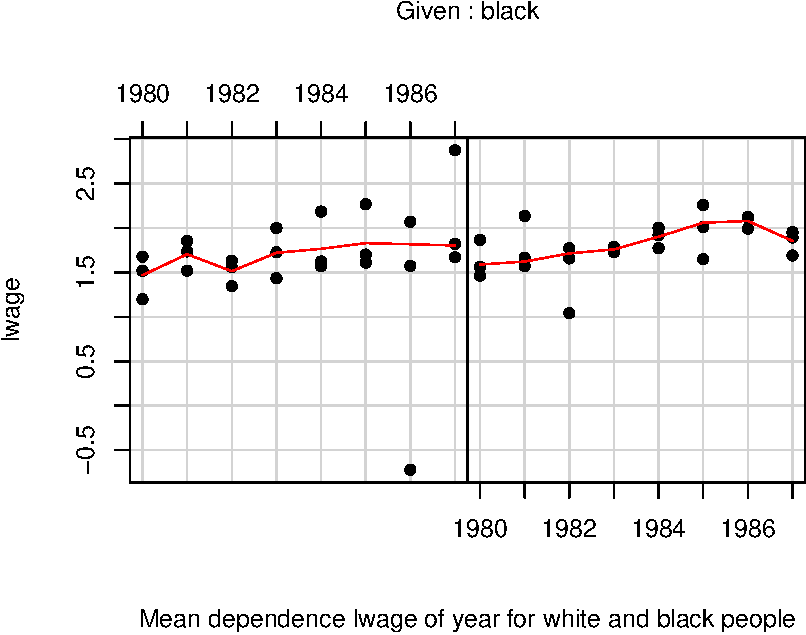
\includegraphics{09-paneldata_files/figure-latex/2 coplot chunk-1.pdf}

Импортируем основной датасет.

\begin{Shaded}
\begin{Highlighting}[]
\NormalTok{Panel =}\StringTok{ }\KeywordTok{import}\NormalTok{(}\StringTok{'lwage_panel_large.csv'}\NormalTok{)}
\end{Highlighting}
\end{Shaded}

Визуализируем гетерогенный эффект. Можно визуализировать по годам или по
индивидам. Здесь уже можно использовать полный датасет. Так как
доверительные интервалы с интервалом в год не пересекаются, можно
увидеть явную гетерогенность.

\begin{Shaded}
\begin{Highlighting}[]
\KeywordTok{plotmeans}\NormalTok{(lwage }\OperatorTok{~}\StringTok{ }\NormalTok{year, }\DataTypeTok{main=}\StringTok{"Heterogeineity across years"}\NormalTok{, }\DataTypeTok{data=}\NormalTok{Panel)}
\end{Highlighting}
\end{Shaded}

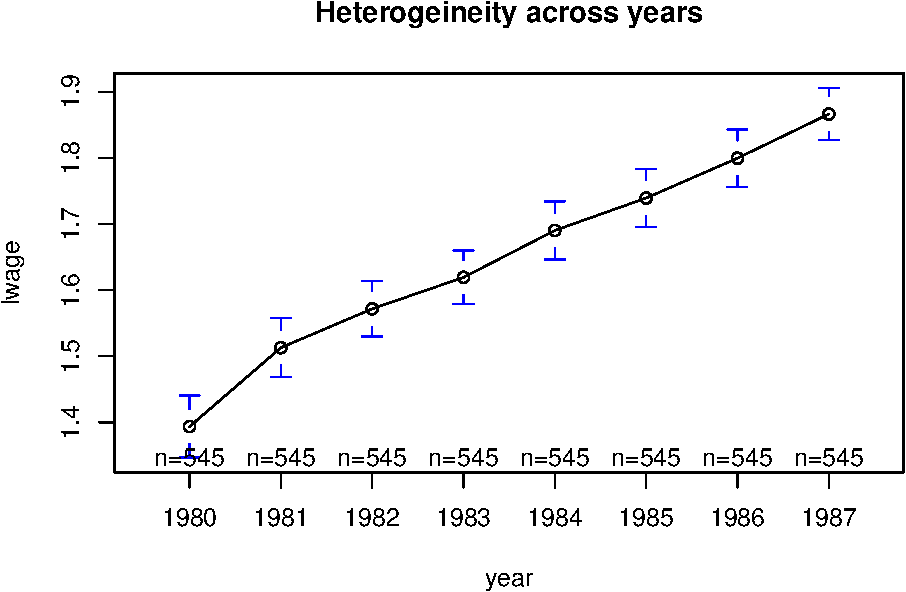
\includegraphics{09-paneldata_files/figure-latex/heterogenity plot-1.pdf}

Модель панельных данных будет выглядеть следующим образом:

\begin{equation}
y_{i t}=\alpha+x_{i t}^{\prime} \beta+z_{i}^{\prime} \gamma+c_{i}+u_{i t}
\end{equation}

где \(\alpha\) -- константа, \(c_{i}\) - индивидуальные эффекты
индивидов, а \(z_i\) -- независимые от времени переменные.
Следовательно, матрица \(X\) - матрица зависимых от времени регрессов,
\(Z\) - матрица независимых от времени регрессоров. Дополнительно
обозначим как \(l_n\) вектор из единиц.

Оценим простую модель с фиксированными эффектами через within-оценку.
Вычитая \(\overline{y}_{i}=1 / T \sum_{t} y_{i t}\) из исходной модели,
получим within-модель:

\begin{equation}
\ddot{y}_{i t}=\ddot{x}_{i t}^{\prime} \beta+\ddot{u}_{i t}
\end{equation}

где
\(\ddot{y}_{i t}=y_{i t}-\overline{y}_{i}, \ddot{x}_{i t k}=x_{i t k}-\overline{x}_{i k}\)
and \(\ddot{u}_{i t}=u_{i t}-\overline{u}_{i}\). Следует заметить, что
константа \(\alpha\), индивидуальные эффекты \(c_i\) и инвариантные ко
времени регрессоры \(z_i\) исчезают из модели.

\begin{equation}
\widehat{\beta}_{F E}=\left(\ddot{X}^{\prime} \ddot{X}\right)^{-1} \ddot{X}^{\prime} \ddot{y}
\end{equation}

\begin{Shaded}
\begin{Highlighting}[]
\NormalTok{ffe =}\StringTok{ }\KeywordTok{plm}\NormalTok{(lwage }\OperatorTok{~}\StringTok{ }\NormalTok{hours, }\DataTypeTok{model=}\StringTok{"within"}\NormalTok{, }\DataTypeTok{data =}\NormalTok{ Panel)}
\KeywordTok{summary}\NormalTok{(ffe)}
\end{Highlighting}
\end{Shaded}

\begin{verbatim}
Oneway (individual) effect Within Model

Call:
plm(formula = lwage ~ hours, data = Panel, model = "within")

Balanced Panel: n = 545, T = 8, N = 4360

Residuals:
     Min.   1st Qu.    Median   3rd Qu.      Max. 
-4.116091 -0.136963  0.015755  0.182507  1.555059 

Coefficients:
         Estimate  Std. Error t-value Pr(>|t|)
hours -5.5854e-07  1.4013e-05 -0.0399   0.9682

Total Sum of Squares:    572.05
Residual Sum of Squares: 572.05
R-Squared:      4.1656e-07
Adj. R-Squared: -0.14289
F-statistic: 0.00158875 on 1 and 3814 DF, p-value: 0.96821
\end{verbatim}

Проверим значимость коэффициентов, используя ковариационную матрицу
ошибок Хубера - Уайта.

\begin{Shaded}
\begin{Highlighting}[]
\KeywordTok{coeftest}\NormalTok{(ffe, }\DataTypeTok{vcov=}\KeywordTok{vcovHC}\NormalTok{(ffe, }\DataTypeTok{cluster=}\StringTok{"group"}\NormalTok{))}
\end{Highlighting}
\end{Shaded}

\begin{verbatim}

t test of coefficients:

         Estimate  Std. Error t value Pr(>|t|)
hours -5.5854e-07  2.5051e-05 -0.0223   0.9822
\end{verbatim}

Оценим модель со случайными эффектами, используя достижимый обобщённый
МНК (FGLS).

\begin{equation}
\left(\begin{array}{c}{\widehat{\alpha}_{R E}} \\ {\widehat{\beta}_{R E}} \\ {\widehat{\gamma}_{R E}}\end{array}\right)=\left(W^{\prime} \widehat{\Omega}_{v}^{-1} W\right)^{-1} W^{\prime} \widehat{\Omega}_{v}^{-1} y
\end{equation}

где

\(W=\left[\iota_{N T} X Z\right] \text { и } \iota_{N T} \text { это вектор из единиц размерности } N T \times 1\)

\begin{Shaded}
\begin{Highlighting}[]
\NormalTok{fre =}\StringTok{ }\KeywordTok{plm}\NormalTok{(lwage }\OperatorTok{~}\StringTok{ }\NormalTok{hours, }\DataTypeTok{model=}\StringTok{"random"}\NormalTok{, }\DataTypeTok{data =}\NormalTok{ Panel)}
\KeywordTok{summary}\NormalTok{(fre)}
\end{Highlighting}
\end{Shaded}

\begin{verbatim}
Oneway (individual) effect Random Effect Model 
   (Swamy-Arora's transformation)

Call:
plm(formula = lwage ~ hours, data = Panel, model = "random")

Balanced Panel: n = 545, T = 8, N = 4360

Effects:
                 var std.dev share
idiosyncratic 0.1500  0.3873 0.528
individual    0.1341  0.3663 0.472
theta: 0.6498

Residuals:
     Min.   1st Qu.    Median   3rd Qu.      Max. 
-4.506028 -0.164365  0.028671  0.218928  1.605623 

Coefficients:
              Estimate Std. Error z-value Pr(>|z|)    
(Intercept) 1.6459e+00 3.3705e-02 48.8332   <2e-16 ***
hours       1.4611e-06 1.3348e-05  0.1095   0.9128    
---
Signif. codes:  0 '***' 0.001 '**' 0.01 '*' 0.05 '.' 0.1 ' ' 1

Total Sum of Squares:    653.53
Residual Sum of Squares: 653.53
R-Squared:      2.7494e-06
Adj. R-Squared: -0.00022671
Chisq: 0.0119818 on 1 DF, p-value: 0.91284
\end{verbatim}

Проверим значимость коэффициентов, используя ковариационную матрицу
ошибок Хубера - Уайта.

\begin{Shaded}
\begin{Highlighting}[]
\KeywordTok{coeftest}\NormalTok{(fre, }\DataTypeTok{vcov=}\KeywordTok{vcovHC}\NormalTok{(ffe, }\DataTypeTok{cluster=}\StringTok{"group"}\NormalTok{))}
\end{Highlighting}
\end{Shaded}

\begin{verbatim}

t test of coefficients:

        Estimate Std. Error t value Pr(>|t|)
hours 1.4611e-06 2.5051e-05  0.0583   0.9535
\end{verbatim}

Проведём тест Хаусмана

\begin{Shaded}
\begin{Highlighting}[]
\KeywordTok{phtest}\NormalTok{(ffe, fre)}
\end{Highlighting}
\end{Shaded}

\begin{verbatim}

    Hausman Test

data:  lwage ~ hours
chisq = 0.22438, df = 1, p-value = 0.6357
alternative hypothesis: one model is inconsistent
\end{verbatim}

Построим FD-оценку.

\begin{equation}
\dot{y}_{i t}=\dot{x}_{i t}^{\prime} \beta+\dot{u}_{i t}
\end{equation}

\(\dot{y}_{i t}=y_{i t}-y_{i, t-1}, \dot{x}_{i t}=x_{i t}-x_{i, t-1}\) и
\(\dot{u}_{i t}=u_{i t}-u_{i, t-1}\)

\begin{Shaded}
\begin{Highlighting}[]
\NormalTok{fd =}\StringTok{ }\KeywordTok{plm}\NormalTok{(lwage }\OperatorTok{~}\StringTok{ }\NormalTok{hours }\OperatorTok{-}\StringTok{ }\DecValTok{1}\NormalTok{, }\DataTypeTok{model=}\StringTok{"fd"}\NormalTok{, }\DataTypeTok{data =}\NormalTok{ Panel)}
\KeywordTok{summary}\NormalTok{(fd)}
\end{Highlighting}
\end{Shaded}

\begin{verbatim}
Oneway (individual) effect First-Difference Model

Call:
plm(formula = lwage ~ hours - 1, data = Panel, model = "fd")

Balanced Panel: n = 545, T = 8, N = 4360
Observations used in estimation: 3815

Residuals:
   Min. 1st Qu.  Median    Mean 3rd Qu.    Max. 
-4.4590 -0.0585  0.0554  0.0793  0.1935  4.7557 

Coefficients:
         Estimate  Std. Error t-value  Pr(>|t|)    
hours -2.0303e-04  1.4585e-05  -13.92 < 2.2e-16 ***
---
Signif. codes:  0 '***' 0.001 '**' 0.01 '*' 0.05 '.' 0.1 ' ' 1

Total Sum of Squares:    751.19
Residual Sum of Squares: 731.45
R-Squared:      0.058688
Adj. R-Squared: 0.058688
F-statistic: 102.938 on 1 and 3814 DF, p-value: < 2.22e-16
\end{verbatim}

Построим LS-оценку с дамми-переменными по каждому индивиду (LSDV).
Видим, что численно её результаты идентичны withih-регрессии, как и
должно быть.

\begin{Shaded}
\begin{Highlighting}[]
\NormalTok{lsdv =}\StringTok{ }\KeywordTok{lm}\NormalTok{(lwage }\OperatorTok{~}\StringTok{ }\NormalTok{hours }\OperatorTok{+}\StringTok{ }\KeywordTok{factor}\NormalTok{(id) }\OperatorTok{-}\StringTok{ }\DecValTok{1}\NormalTok{, }\DataTypeTok{data=}\NormalTok{Panel)}
\KeywordTok{summary}\NormalTok{(lsdv)}
\end{Highlighting}
\end{Shaded}

\begin{verbatim}

Call:
lm(formula = lwage ~ hours + factor(id) - 1, data = Panel)

Residuals:
    Min      1Q  Median      3Q     Max 
-4.1161 -0.1370  0.0158  0.1825  1.5551 

Coefficients:
                Estimate Std. Error t value Pr(>|t|)    
hours         -5.585e-07  1.401e-05  -0.040 0.968208    
factor(id)1    1.257e+00  1.425e-01   8.825  < 2e-16 ***
factor(id)2    1.639e+00  1.413e-01  11.597  < 2e-16 ***
factor(id)3    2.036e+00  1.408e-01  14.455  < 2e-16 ***
factor(id)4    1.775e+00  1.404e-01  12.639  < 2e-16 ***
factor(id)5    2.056e+00  1.401e-01  14.680  < 2e-16 ***
factor(id)6    1.435e+00  1.424e-01  10.076  < 2e-16 ***
factor(id)7    1.996e+00  1.418e-01  14.077  < 2e-16 ***
factor(id)8    1.065e+00  1.434e-01   7.426 1.37e-13 ***
factor(id)9    1.474e+00  1.398e-01  10.537  < 2e-16 ***
factor(id)10   1.395e+00  1.394e-01  10.005  < 2e-16 ***
factor(id)11   1.385e+00  1.378e-01  10.052  < 2e-16 ***
factor(id)12   2.193e+00  1.396e-01  15.711  < 2e-16 ***
factor(id)13   1.840e+00  1.404e-01  13.103  < 2e-16 ***
factor(id)14   2.060e+00  1.413e-01  14.581  < 2e-16 ***
factor(id)15   2.455e+00  1.405e-01  17.468  < 2e-16 ***
factor(id)16   1.675e+00  1.400e-01  11.963  < 2e-16 ***
factor(id)17   1.697e+00  1.411e-01  12.031  < 2e-16 ***
factor(id)18   2.033e+00  1.398e-01  14.544  < 2e-16 ***
factor(id)19   2.214e+00  1.425e-01  15.533  < 2e-16 ***
factor(id)20   1.525e+00  1.400e-01  10.896  < 2e-16 ***
factor(id)21   1.726e+00  1.401e-01  12.321  < 2e-16 ***
factor(id)22   1.769e+00  1.400e-01  12.635  < 2e-16 ***
factor(id)23   2.077e+00  1.408e-01  14.754  < 2e-16 ***
factor(id)24   2.368e+00  1.400e-01  16.919  < 2e-16 ***
factor(id)25   1.311e+00  1.443e-01   9.085  < 2e-16 ***
factor(id)26   1.700e+00  1.399e-01  12.153  < 2e-16 ***
factor(id)27   2.284e+00  1.409e-01  16.214  < 2e-16 ***
factor(id)28   1.411e+00  1.411e-01  10.000  < 2e-16 ***
factor(id)29   7.640e-01  1.412e-01   5.409 6.71e-08 ***
factor(id)30   1.950e+00  1.403e-01  13.895  < 2e-16 ***
factor(id)31   1.670e+00  1.402e-01  11.917  < 2e-16 ***
factor(id)32   1.928e+00  1.407e-01  13.709  < 2e-16 ***
factor(id)33   2.362e+00  1.396e-01  16.918  < 2e-16 ***
factor(id)34   1.098e+00  1.409e-01   7.791 8.49e-15 ***
factor(id)35   2.103e+00  1.402e-01  14.995  < 2e-16 ***
factor(id)36   1.657e+00  1.402e-01  11.816  < 2e-16 ***
factor(id)37   1.664e+00  1.416e-01  11.753  < 2e-16 ***
factor(id)38   1.694e+00  1.406e-01  12.045  < 2e-16 ***
factor(id)39   2.063e+00  1.416e-01  14.576  < 2e-16 ***
factor(id)40   1.657e+00  1.400e-01  11.833  < 2e-16 ***
factor(id)41   5.381e-01  1.386e-01   3.883 0.000105 ***
factor(id)42   7.392e-01  1.390e-01   5.319 1.10e-07 ***
factor(id)43   1.713e+00  1.388e-01  12.345  < 2e-16 ***
factor(id)44   1.782e+00  1.408e-01  12.660  < 2e-16 ***
factor(id)45   1.989e+00  1.399e-01  14.215  < 2e-16 ***
factor(id)46   1.763e+00  1.413e-01  12.476  < 2e-16 ***
factor(id)47   1.128e+00  1.393e-01   8.095 7.63e-16 ***
factor(id)48   2.019e+00  1.416e-01  14.260  < 2e-16 ***
factor(id)49   8.453e-01  1.383e-01   6.112 1.08e-09 ***
factor(id)50   1.874e+00  1.409e-01  13.301  < 2e-16 ***
factor(id)51   1.759e+00  1.391e-01  12.644  < 2e-16 ***
factor(id)52   1.487e+00  1.397e-01  10.648  < 2e-16 ***
factor(id)53   2.212e+00  1.413e-01  15.658  < 2e-16 ***
factor(id)54   1.182e+00  1.391e-01   8.494  < 2e-16 ***
factor(id)55   2.022e+00  1.403e-01  14.411  < 2e-16 ***
factor(id)56   1.301e+00  1.390e-01   9.354  < 2e-16 ***
factor(id)57   1.353e+00  1.420e-01   9.525  < 2e-16 ***
factor(id)58   2.352e+00  1.406e-01  16.729  < 2e-16 ***
factor(id)59   2.146e+00  1.398e-01  15.346  < 2e-16 ***
factor(id)60   1.435e+00  1.400e-01  10.249  < 2e-16 ***
factor(id)61   1.250e+00  1.436e-01   8.703  < 2e-16 ***
factor(id)62   2.068e+00  1.402e-01  14.756  < 2e-16 ***
factor(id)63   1.305e+00  1.410e-01   9.257  < 2e-16 ***
factor(id)64   1.965e+00  1.404e-01  13.994  < 2e-16 ***
factor(id)65   1.374e+00  1.395e-01   9.852  < 2e-16 ***
factor(id)66   1.379e+00  1.421e-01   9.704  < 2e-16 ***
factor(id)67   1.181e+00  1.415e-01   8.346  < 2e-16 ***
factor(id)68   1.779e+00  1.401e-01  12.702  < 2e-16 ***
factor(id)69   1.157e+00  1.439e-01   8.040 1.19e-15 ***
factor(id)70   2.089e+00  1.387e-01  15.058  < 2e-16 ***
factor(id)71   2.081e+00  1.403e-01  14.829  < 2e-16 ***
factor(id)72   1.780e+00  1.400e-01  12.714  < 2e-16 ***
factor(id)73   1.927e+00  1.405e-01  13.716  < 2e-16 ***
factor(id)74   1.546e+00  1.395e-01  11.084  < 2e-16 ***
factor(id)75   1.874e+00  1.402e-01  13.369  < 2e-16 ***
factor(id)76   1.319e+00  1.397e-01   9.444  < 2e-16 ***
factor(id)77   1.935e+00  1.400e-01  13.819  < 2e-16 ***
factor(id)78   1.469e+00  1.420e-01  10.343  < 2e-16 ***
factor(id)79   1.782e+00  1.393e-01  12.792  < 2e-16 ***
factor(id)80   1.677e+00  1.484e-01  11.304  < 2e-16 ***
factor(id)81   2.016e+00  1.399e-01  14.405  < 2e-16 ***
factor(id)82   1.291e+00  1.407e-01   9.175  < 2e-16 ***
factor(id)83   1.650e+00  1.410e-01  11.707  < 2e-16 ***
factor(id)84   1.710e+00  1.400e-01  12.214  < 2e-16 ***
factor(id)85   1.194e+00  1.413e-01   8.452  < 2e-16 ***
factor(id)86   1.491e+00  1.399e-01  10.661  < 2e-16 ***
factor(id)87   1.049e+00  1.426e-01   7.354 2.35e-13 ***
factor(id)88   1.215e+00  1.401e-01   8.669  < 2e-16 ***
factor(id)89   1.492e+00  1.406e-01  10.612  < 2e-16 ***
factor(id)90   1.429e+00  1.413e-01  10.115  < 2e-16 ***
factor(id)91   1.206e+00  1.396e-01   8.640  < 2e-16 ***
factor(id)92   1.558e+00  1.406e-01  11.082  < 2e-16 ***
factor(id)93   1.751e+00  1.422e-01  12.312  < 2e-16 ***
factor(id)94   1.728e+00  1.402e-01  12.327  < 2e-16 ***
factor(id)95   1.573e+00  1.398e-01  11.250  < 2e-16 ***
factor(id)96   2.075e+00  1.401e-01  14.812  < 2e-16 ***
factor(id)97   1.526e+00  1.400e-01  10.897  < 2e-16 ***
factor(id)98   1.874e+00  1.407e-01  13.318  < 2e-16 ***
factor(id)99   1.741e+00  1.396e-01  12.472  < 2e-16 ***
factor(id)100  2.157e+00  1.400e-01  15.408  < 2e-16 ***
factor(id)101  2.087e+00  1.402e-01  14.887  < 2e-16 ***
factor(id)102  1.832e+00  1.390e-01  13.178  < 2e-16 ***
factor(id)103  1.072e+00  1.386e-01   7.736 1.31e-14 ***
factor(id)104  1.393e+00  1.408e-01   9.898  < 2e-16 ***
factor(id)105  2.552e+00  1.401e-01  18.215  < 2e-16 ***
factor(id)106  1.115e+00  1.396e-01   7.989 1.78e-15 ***
factor(id)107  1.900e+00  1.402e-01  13.545  < 2e-16 ***
factor(id)108  1.339e+00  1.400e-01   9.565  < 2e-16 ***
factor(id)109  1.707e+00  1.410e-01  12.101  < 2e-16 ***
factor(id)110  1.452e+00  1.387e-01  10.469  < 2e-16 ***
factor(id)111  1.853e+00  1.417e-01  13.073  < 2e-16 ***
factor(id)112  1.700e+00  1.421e-01  11.964  < 2e-16 ***
factor(id)113  1.997e+00  1.394e-01  14.327  < 2e-16 ***
factor(id)114  1.143e+00  1.402e-01   8.152 4.79e-16 ***
factor(id)115  1.835e+00  1.418e-01  12.945  < 2e-16 ***
factor(id)116  1.515e+00  1.397e-01  10.847  < 2e-16 ***
factor(id)117  1.679e+00  1.443e-01  11.635  < 2e-16 ***
factor(id)118  1.374e+00  1.379e-01   9.969  < 2e-16 ***
factor(id)119  1.982e+00  1.402e-01  14.130  < 2e-16 ***
factor(id)120  2.333e+00  1.403e-01  16.626  < 2e-16 ***
factor(id)121  1.764e+00  1.398e-01  12.620  < 2e-16 ***
factor(id)122  1.698e+00  1.394e-01  12.180  < 2e-16 ***
factor(id)123  2.116e+00  1.409e-01  15.022  < 2e-16 ***
factor(id)124  3.344e-01  1.394e-01   2.398 0.016514 *  
factor(id)125  1.083e+00  1.414e-01   7.658 2.37e-14 ***
factor(id)126  2.279e+00  1.400e-01  16.280  < 2e-16 ***
factor(id)127  1.372e+00  1.400e-01   9.804  < 2e-16 ***
factor(id)128  1.629e+00  1.398e-01  11.650  < 2e-16 ***
factor(id)129  1.669e+00  1.409e-01  11.845  < 2e-16 ***
factor(id)130  1.826e+00  1.423e-01  12.831  < 2e-16 ***
factor(id)131  2.243e+00  1.405e-01  15.960  < 2e-16 ***
factor(id)132  1.448e+00  1.399e-01  10.349  < 2e-16 ***
factor(id)133  1.154e+00  1.396e-01   8.261  < 2e-16 ***
factor(id)134  1.131e+00  1.392e-01   8.125 5.97e-16 ***
factor(id)135  2.035e+00  1.405e-01  14.485  < 2e-16 ***
factor(id)136  2.016e+00  1.405e-01  14.348  < 2e-16 ***
factor(id)137  1.839e+00  1.401e-01  13.131  < 2e-16 ***
factor(id)138  1.489e+00  1.399e-01  10.644  < 2e-16 ***
factor(id)139  1.736e+00  1.399e-01  12.413  < 2e-16 ***
factor(id)140  1.241e+00  1.390e-01   8.926  < 2e-16 ***
factor(id)141  1.067e+00  1.392e-01   7.668 2.21e-14 ***
factor(id)142  1.717e+00  1.404e-01  12.227  < 2e-16 ***
factor(id)143  2.174e+00  1.403e-01  15.494  < 2e-16 ***
factor(id)144  1.199e+00  1.455e-01   8.241 2.32e-16 ***
factor(id)145  1.574e+00  1.409e-01  11.171  < 2e-16 ***
factor(id)146  1.834e+00  1.411e-01  12.991  < 2e-16 ***
factor(id)147  1.319e+00  1.400e-01   9.422  < 2e-16 ***
factor(id)148  2.021e+00  1.401e-01  14.424  < 2e-16 ***
factor(id)149  1.622e+00  1.403e-01  11.567  < 2e-16 ***
factor(id)150  1.163e+00  1.407e-01   8.270  < 2e-16 ***
factor(id)151  2.226e+00  1.400e-01  15.900  < 2e-16 ***
factor(id)152  1.304e+00  1.416e-01   9.208  < 2e-16 ***
factor(id)153  2.283e+00  1.402e-01  16.290  < 2e-16 ***
factor(id)154  1.108e+00  1.403e-01   7.893 3.83e-15 ***
factor(id)155  9.691e-01  1.413e-01   6.860 8.00e-12 ***
factor(id)156  1.453e+00  1.400e-01  10.378  < 2e-16 ***
factor(id)157  1.716e+00  1.398e-01  12.279  < 2e-16 ***
factor(id)158  1.617e+00  1.405e-01  11.510  < 2e-16 ***
factor(id)159  2.082e+00  1.392e-01  14.963  < 2e-16 ***
factor(id)160  1.294e+00  1.400e-01   9.241  < 2e-16 ***
factor(id)161  1.464e+00  1.401e-01  10.445  < 2e-16 ***
factor(id)162  1.863e+00  1.407e-01  13.247  < 2e-16 ***
factor(id)163  1.778e+00  1.399e-01  12.708  < 2e-16 ***
factor(id)164  2.002e+00  1.396e-01  14.341  < 2e-16 ***
factor(id)165  1.891e+00  1.422e-01  13.297  < 2e-16 ***
factor(id)166  2.150e+00  1.395e-01  15.414  < 2e-16 ***
factor(id)167  1.067e+00  1.392e-01   7.662 2.31e-14 ***
factor(id)168  1.539e+00  1.387e-01  11.100  < 2e-16 ***
factor(id)169  1.196e+00  1.400e-01   8.548  < 2e-16 ***
factor(id)170  1.568e+00  1.395e-01  11.244  < 2e-16 ***
factor(id)171  1.674e+00  1.426e-01  11.740  < 2e-16 ***
factor(id)172  1.751e+00  1.411e-01  12.407  < 2e-16 ***
factor(id)173  2.264e+00  1.408e-01  16.077  < 2e-16 ***
factor(id)174  2.221e+00  1.402e-01  15.842  < 2e-16 ***
factor(id)175  1.775e+00  1.414e-01  12.547  < 2e-16 ***
factor(id)176  2.361e+00  1.400e-01  16.867  < 2e-16 ***
factor(id)177  1.784e+00  1.407e-01  12.680  < 2e-16 ***
factor(id)178  9.877e-01  1.407e-01   7.018 2.66e-12 ***
factor(id)179  7.941e-01  1.395e-01   5.691 1.36e-08 ***
factor(id)180  1.910e+00  1.400e-01  13.646  < 2e-16 ***
factor(id)181  2.093e+00  1.398e-01  14.972  < 2e-16 ***
factor(id)182  1.775e+00  1.393e-01  12.741  < 2e-16 ***
factor(id)183  2.011e+00  1.406e-01  14.302  < 2e-16 ***
factor(id)184  1.898e+00  1.398e-01  13.575  < 2e-16 ***
factor(id)185  1.884e+00  1.410e-01  13.361  < 2e-16 ***
factor(id)186  1.606e+00  1.392e-01  11.537  < 2e-16 ***
factor(id)187  1.841e+00  1.401e-01  13.143  < 2e-16 ***
factor(id)188  1.578e+00  1.405e-01  11.230  < 2e-16 ***
factor(id)189  2.079e+00  1.402e-01  14.825  < 2e-16 ***
factor(id)190  1.963e+00  1.386e-01  14.161  < 2e-16 ***
factor(id)191  1.444e+00  1.392e-01  10.373  < 2e-16 ***
factor(id)192  1.462e+00  1.400e-01  10.438  < 2e-16 ***
factor(id)193  1.786e+00  1.386e-01  12.892  < 2e-16 ***
factor(id)194  1.390e+00  1.409e-01   9.864  < 2e-16 ***
factor(id)195  8.809e-01  1.375e-01   6.406 1.68e-10 ***
factor(id)196  1.660e+00  1.403e-01  11.831  < 2e-16 ***
factor(id)197  1.788e+00  1.386e-01  12.904  < 2e-16 ***
factor(id)198  1.813e+00  1.393e-01  13.015  < 2e-16 ***
factor(id)199  1.740e+00  1.399e-01  12.436  < 2e-16 ***
factor(id)200  1.730e+00  1.393e-01  12.424  < 2e-16 ***
factor(id)201  2.524e+00  1.395e-01  18.096  < 2e-16 ***
factor(id)202  1.174e+00  1.393e-01   8.432  < 2e-16 ***
factor(id)203  1.215e+00  1.393e-01   8.726  < 2e-16 ***
factor(id)204  1.746e+00  1.411e-01  12.378  < 2e-16 ***
factor(id)205  1.806e+00  1.406e-01  12.839  < 2e-16 ***
factor(id)206  1.829e+00  1.419e-01  12.888  < 2e-16 ***
factor(id)207  1.874e+00  1.398e-01  13.401  < 2e-16 ***
factor(id)208  1.621e+00  1.405e-01  11.539  < 2e-16 ***
factor(id)209  1.965e+00  1.407e-01  13.968  < 2e-16 ***
factor(id)210  1.496e+00  1.395e-01  10.719  < 2e-16 ***
factor(id)211  1.063e+00  1.395e-01   7.623 3.12e-14 ***
factor(id)212  1.906e+00  1.406e-01  13.558  < 2e-16 ***
factor(id)213  1.442e+00  1.402e-01  10.284  < 2e-16 ***
factor(id)214  2.195e+00  1.404e-01  15.638  < 2e-16 ***
factor(id)215  1.597e+00  1.398e-01  11.425  < 2e-16 ***
factor(id)216  2.107e+00  1.400e-01  15.050  < 2e-16 ***
factor(id)217  2.296e+00  1.382e-01  16.612  < 2e-16 ***
factor(id)218  1.735e+00  1.399e-01  12.400  < 2e-16 ***
factor(id)219  2.044e+00  1.399e-01  14.608  < 2e-16 ***
factor(id)220  1.842e+00  1.399e-01  13.167  < 2e-16 ***
factor(id)221  2.098e+00  1.400e-01  14.987  < 2e-16 ***
factor(id)222  1.562e+00  1.399e-01  11.162  < 2e-16 ***
factor(id)223  1.889e+00  1.390e-01  13.597  < 2e-16 ***
factor(id)224  1.609e+00  1.411e-01  11.405  < 2e-16 ***
factor(id)225  1.953e+00  1.403e-01  13.917  < 2e-16 ***
factor(id)226  2.024e+00  1.412e-01  14.331  < 2e-16 ***
factor(id)227  2.148e+00  1.406e-01  15.282  < 2e-16 ***
factor(id)228  7.610e-01  1.389e-01   5.478 4.57e-08 ***
factor(id)229  1.648e+00  1.401e-01  11.765  < 2e-16 ***
factor(id)230  2.164e+00  1.424e-01  15.196  < 2e-16 ***
factor(id)231  1.953e+00  1.410e-01  13.854  < 2e-16 ***
factor(id)232  1.717e+00  1.404e-01  12.229  < 2e-16 ***
factor(id)233  1.791e+00  1.400e-01  12.799  < 2e-16 ***
factor(id)234  1.924e+00  1.408e-01  13.665  < 2e-16 ***
factor(id)235  1.877e+00  1.398e-01  13.423  < 2e-16 ***
factor(id)236  2.054e+00  1.402e-01  14.649  < 2e-16 ***
factor(id)237  1.377e+00  1.398e-01   9.851  < 2e-16 ***
factor(id)238  1.642e+00  1.405e-01  11.686  < 2e-16 ***
factor(id)239  2.352e+00  1.396e-01  16.854  < 2e-16 ***
factor(id)240  1.858e+00  1.403e-01  13.241  < 2e-16 ***
factor(id)241  1.303e+00  1.391e-01   9.368  < 2e-16 ***
factor(id)242  1.721e+00  1.422e-01  12.104  < 2e-16 ***
factor(id)243  1.643e+00  1.402e-01  11.713  < 2e-16 ***
factor(id)244  2.042e+00  1.400e-01  14.583  < 2e-16 ***
factor(id)245  1.352e+00  1.398e-01   9.667  < 2e-16 ***
factor(id)246  1.419e+00  1.413e-01  10.046  < 2e-16 ***
factor(id)247  1.495e+00  1.424e-01  10.497  < 2e-16 ***
factor(id)248  2.519e+00  1.403e-01  17.953  < 2e-16 ***
factor(id)249  2.531e+00  1.399e-01  18.087  < 2e-16 ***
factor(id)250  2.048e+00  1.400e-01  14.625  < 2e-16 ***
factor(id)251  1.288e+00  1.394e-01   9.241  < 2e-16 ***
factor(id)252  1.428e+00  1.407e-01  10.146  < 2e-16 ***
factor(id)253  1.873e+00  1.402e-01  13.362  < 2e-16 ***
factor(id)254  1.410e+00  1.402e-01  10.056  < 2e-16 ***
factor(id)255  1.509e+00  1.418e-01  10.643  < 2e-16 ***
factor(id)256  1.993e+00  1.403e-01  14.209  < 2e-16 ***
factor(id)257  1.911e+00  1.396e-01  13.689  < 2e-16 ***
factor(id)258  1.184e+00  1.415e-01   8.367  < 2e-16 ***
factor(id)259  1.773e+00  1.404e-01  12.632  < 2e-16 ***
factor(id)260  1.772e+00  1.427e-01  12.417  < 2e-16 ***
factor(id)261  1.071e+00  1.380e-01   7.758 1.10e-14 ***
factor(id)262  1.814e+00  1.404e-01  12.920  < 2e-16 ***
factor(id)263  1.300e+00  1.401e-01   9.278  < 2e-16 ***
factor(id)264  8.232e-01  1.385e-01   5.945 3.00e-09 ***
factor(id)265  1.521e+00  1.399e-01  10.873  < 2e-16 ***
factor(id)266  1.735e+00  1.395e-01  12.434  < 2e-16 ***
factor(id)267  1.191e+00  1.401e-01   8.501  < 2e-16 ***
factor(id)268  2.020e+00  1.408e-01  14.341  < 2e-16 ***
factor(id)269  1.939e+00  1.393e-01  13.917  < 2e-16 ***
factor(id)270  1.853e+00  1.390e-01  13.332  < 2e-16 ***
factor(id)271  1.393e+00  1.407e-01   9.899  < 2e-16 ***
factor(id)272  1.303e+00  1.402e-01   9.297  < 2e-16 ***
factor(id)273  2.135e+00  1.395e-01  15.303  < 2e-16 ***
factor(id)274  2.009e+00  1.397e-01  14.385  < 2e-16 ***
factor(id)275  1.382e+00  1.384e-01   9.988  < 2e-16 ***
factor(id)276  1.666e+00  1.416e-01  11.764  < 2e-16 ***
factor(id)277  1.320e+00  1.401e-01   9.420  < 2e-16 ***
factor(id)278  2.165e+00  1.400e-01  15.461  < 2e-16 ***
factor(id)279  1.372e+00  1.408e-01   9.739  < 2e-16 ***
factor(id)280  2.221e+00  1.400e-01  15.865  < 2e-16 ***
factor(id)281  1.767e+00  1.401e-01  12.611  < 2e-16 ***
factor(id)282  1.782e+00  1.414e-01  12.605  < 2e-16 ***
factor(id)283  1.311e+00  1.405e-01   9.333  < 2e-16 ***
factor(id)284  1.324e+00  1.402e-01   9.445  < 2e-16 ***
factor(id)285  1.051e+00  1.384e-01   7.598 3.75e-14 ***
factor(id)286  2.216e+00  1.398e-01  15.852  < 2e-16 ***
factor(id)287  1.226e+00  1.391e-01   8.816  < 2e-16 ***
factor(id)288  2.122e+00  1.400e-01  15.159  < 2e-16 ***
factor(id)289  1.599e+00  1.402e-01  11.407  < 2e-16 ***
factor(id)290  1.647e+00  1.403e-01  11.737  < 2e-16 ***
factor(id)291  1.373e+00  1.431e-01   9.594  < 2e-16 ***
factor(id)292  1.399e+00  1.400e-01   9.996  < 2e-16 ***
factor(id)293  1.120e+00  1.406e-01   7.965 2.17e-15 ***
factor(id)294  1.582e+00  1.409e-01  11.222  < 2e-16 ***
factor(id)295  1.179e+00  1.394e-01   8.456  < 2e-16 ***
factor(id)296  2.352e+00  1.403e-01  16.762  < 2e-16 ***
factor(id)297  2.279e+00  1.402e-01  16.257  < 2e-16 ***
factor(id)298  1.466e+00  1.433e-01  10.229  < 2e-16 ***
factor(id)299  1.836e+00  1.409e-01  13.033  < 2e-16 ***
factor(id)300  1.953e+00  1.407e-01  13.882  < 2e-16 ***
factor(id)301  2.216e+00  1.409e-01  15.728  < 2e-16 ***
factor(id)302  1.850e+00  1.399e-01  13.224  < 2e-16 ***
factor(id)303  1.739e+00  1.398e-01  12.446  < 2e-16 ***
factor(id)304  1.619e+00  1.414e-01  11.450  < 2e-16 ***
factor(id)305  1.650e+00  1.402e-01  11.768  < 2e-16 ***
factor(id)306  1.390e+00  1.415e-01   9.825  < 2e-16 ***
factor(id)307  1.322e+00  1.417e-01   9.329  < 2e-16 ***
factor(id)308  1.667e+00  1.404e-01  11.877  < 2e-16 ***
factor(id)309  2.002e+00  1.413e-01  14.169  < 2e-16 ***
factor(id)310  1.502e+00  1.416e-01  10.609  < 2e-16 ***
factor(id)311  1.434e+00  1.401e-01  10.232  < 2e-16 ***
factor(id)312  9.779e-01  1.396e-01   7.005 2.90e-12 ***
factor(id)313  1.342e+00  1.400e-01   9.584  < 2e-16 ***
factor(id)314  1.577e+00  1.397e-01  11.291  < 2e-16 ***
factor(id)315  1.530e+00  1.418e-01  10.784  < 2e-16 ***
factor(id)316  1.352e+00  1.395e-01   9.688  < 2e-16 ***
factor(id)317  1.258e+00  1.409e-01   8.925  < 2e-16 ***
factor(id)318  1.507e+00  1.413e-01  10.664  < 2e-16 ***
factor(id)319  1.437e+00  1.418e-01  10.133  < 2e-16 ***
factor(id)320  1.315e+00  1.406e-01   9.352  < 2e-16 ***
factor(id)321  1.680e+00  1.398e-01  12.014  < 2e-16 ***
factor(id)322  1.927e+00  1.414e-01  13.630  < 2e-16 ***
factor(id)323  1.447e+00  1.397e-01  10.358  < 2e-16 ***
factor(id)324  1.653e+00  1.420e-01  11.644  < 2e-16 ***
factor(id)325  1.805e+00  1.397e-01  12.921  < 2e-16 ***
factor(id)326  1.572e+00  1.401e-01  11.218  < 2e-16 ***
factor(id)327  1.948e+00  1.410e-01  13.818  < 2e-16 ***
factor(id)328  1.317e+00  1.409e-01   9.350  < 2e-16 ***
factor(id)329  1.777e+00  1.403e-01  12.663  < 2e-16 ***
factor(id)330  1.847e+00  1.397e-01  13.224  < 2e-16 ***
factor(id)331  1.914e+00  1.396e-01  13.709  < 2e-16 ***
factor(id)332  1.518e+00  1.400e-01  10.842  < 2e-16 ***
factor(id)333  1.725e+00  1.400e-01  12.320  < 2e-16 ***
factor(id)334  1.673e+00  1.399e-01  11.956  < 2e-16 ***
factor(id)335  1.233e+00  1.424e-01   8.661  < 2e-16 ***
factor(id)336  1.373e+00  1.402e-01   9.793  < 2e-16 ***
factor(id)337  1.249e+00  1.406e-01   8.888  < 2e-16 ***
factor(id)338  1.307e+00  1.391e-01   9.399  < 2e-16 ***
factor(id)339  1.633e+00  1.406e-01  11.615  < 2e-16 ***
factor(id)340  1.669e+00  1.397e-01  11.942  < 2e-16 ***
factor(id)341  1.989e+00  1.400e-01  14.209  < 2e-16 ***
factor(id)342  7.782e-01  1.417e-01   5.492 4.24e-08 ***
factor(id)343  7.649e-01  1.399e-01   5.466 4.89e-08 ***
factor(id)344  1.091e+00  1.401e-01   7.782 9.09e-15 ***
factor(id)345  1.593e+00  1.429e-01  11.149  < 2e-16 ***
factor(id)346  1.717e+00  1.401e-01  12.250  < 2e-16 ***
factor(id)347  1.800e+00  1.401e-01  12.846  < 2e-16 ***
factor(id)348  1.450e+00  1.395e-01  10.400  < 2e-16 ***
factor(id)349  1.851e+00  1.402e-01  13.208  < 2e-16 ***
factor(id)350  1.161e+00  1.392e-01   8.345  < 2e-16 ***
factor(id)351  2.047e+00  1.399e-01  14.632  < 2e-16 ***
factor(id)352  1.816e+00  1.406e-01  12.923  < 2e-16 ***
factor(id)353  2.172e+00  1.409e-01  15.414  < 2e-16 ***
factor(id)354  1.244e+00  1.398e-01   8.896  < 2e-16 ***
factor(id)355  2.019e+00  1.401e-01  14.415  < 2e-16 ***
factor(id)356  1.467e+00  1.400e-01  10.476  < 2e-16 ***
factor(id)357  1.600e+00  1.400e-01  11.430  < 2e-16 ***
factor(id)358  1.302e+00  1.415e-01   9.202  < 2e-16 ***
factor(id)359  1.698e+00  1.408e-01  12.057  < 2e-16 ***
factor(id)360  1.807e+00  1.408e-01  12.832  < 2e-16 ***
factor(id)361  1.837e+00  1.451e-01  12.660  < 2e-16 ***
factor(id)362  1.482e+00  1.394e-01  10.630  < 2e-16 ***
factor(id)363  2.686e+00  1.407e-01  19.096  < 2e-16 ***
factor(id)364  2.075e+00  1.400e-01  14.817  < 2e-16 ***
factor(id)365  1.734e+00  1.400e-01  12.387  < 2e-16 ***
factor(id)366  1.715e+00  1.400e-01  12.248  < 2e-16 ***
factor(id)367  1.018e+00  1.395e-01   7.297 3.55e-13 ***
factor(id)368  1.391e+00  1.394e-01   9.979  < 2e-16 ***
factor(id)369  1.410e+00  1.400e-01  10.071  < 2e-16 ***
factor(id)370  1.409e+00  1.397e-01  10.081  < 2e-16 ***
factor(id)371  1.666e+00  1.410e-01  11.815  < 2e-16 ***
factor(id)372  1.219e+00  1.407e-01   8.665  < 2e-16 ***
factor(id)373  1.963e+00  1.396e-01  14.061  < 2e-16 ***
factor(id)374  1.415e+00  1.413e-01  10.013  < 2e-16 ***
factor(id)375  1.925e+00  1.403e-01  13.718  < 2e-16 ***
factor(id)376  1.605e+00  1.414e-01  11.358  < 2e-16 ***
factor(id)377  1.592e+00  1.422e-01  11.194  < 2e-16 ***
factor(id)378  1.783e+00  1.400e-01  12.734  < 2e-16 ***
factor(id)379  1.309e+00  1.440e-01   9.088  < 2e-16 ***
factor(id)380  1.897e+00  1.410e-01  13.452  < 2e-16 ***
factor(id)381  1.581e+00  1.387e-01  11.406  < 2e-16 ***
factor(id)382  3.175e+00  1.393e-01  22.796  < 2e-16 ***
factor(id)383  1.219e+00  1.389e-01   8.775  < 2e-16 ***
factor(id)384  1.769e+00  1.411e-01  12.532  < 2e-16 ***
factor(id)385  2.302e+00  1.405e-01  16.388  < 2e-16 ***
factor(id)386  1.732e+00  1.403e-01  12.346  < 2e-16 ***
factor(id)387  2.297e+00  1.400e-01  16.409  < 2e-16 ***
factor(id)388  1.802e+00  1.400e-01  12.867  < 2e-16 ***
factor(id)389  2.019e+00  1.410e-01  14.323  < 2e-16 ***
factor(id)390  1.593e+00  1.400e-01  11.381  < 2e-16 ***
factor(id)391  1.384e+00  1.401e-01   9.878  < 2e-16 ***
factor(id)392  2.439e+00  1.409e-01  17.310  < 2e-16 ***
factor(id)393  1.571e+00  1.402e-01  11.200  < 2e-16 ***
factor(id)394  1.505e+00  1.401e-01  10.745  < 2e-16 ***
factor(id)395  1.448e+00  1.402e-01  10.330  < 2e-16 ***
factor(id)396  1.377e+00  1.407e-01   9.783  < 2e-16 ***
factor(id)397  1.845e+00  1.402e-01  13.162  < 2e-16 ***
factor(id)398  1.497e+00  1.398e-01  10.710  < 2e-16 ***
factor(id)399  2.313e+00  1.408e-01  16.434  < 2e-16 ***
factor(id)400  1.224e+00  1.409e-01   8.690  < 2e-16 ***
factor(id)401  1.804e+00  1.416e-01  12.739  < 2e-16 ***
factor(id)402  2.198e+00  1.405e-01  15.648  < 2e-16 ***
factor(id)403  1.715e+00  1.400e-01  12.244  < 2e-16 ***
factor(id)404  1.699e+00  1.408e-01  12.069  < 2e-16 ***
factor(id)405  1.531e+00  1.397e-01  10.964  < 2e-16 ***
factor(id)406  2.051e+00  1.400e-01  14.650  < 2e-16 ***
factor(id)407  1.423e+00  1.411e-01  10.085  < 2e-16 ***
factor(id)408  1.456e+00  1.431e-01  10.177  < 2e-16 ***
factor(id)409  1.566e+00  1.400e-01  11.184  < 2e-16 ***
factor(id)410  1.326e+00  1.392e-01   9.530  < 2e-16 ***
factor(id)411  1.088e+00  1.393e-01   7.815 7.08e-15 ***
factor(id)412  9.472e-01  1.398e-01   6.774 1.45e-11 ***
factor(id)413  2.315e+00  1.398e-01  16.562  < 2e-16 ***
factor(id)414  8.820e-01  1.448e-01   6.092 1.23e-09 ***
factor(id)415  1.235e+00  1.398e-01   8.837  < 2e-16 ***
factor(id)416  1.254e+00  1.398e-01   8.968  < 2e-16 ***
factor(id)417  1.849e+00  1.403e-01  13.180  < 2e-16 ***
factor(id)418  1.394e+00  1.419e-01   9.825  < 2e-16 ***
factor(id)419  9.013e-01  1.407e-01   6.407 1.67e-10 ***
factor(id)420  1.391e+00  1.405e-01   9.900  < 2e-16 ***
factor(id)421  7.832e-01  1.400e-01   5.595 2.36e-08 ***
factor(id)422  1.735e+00  1.396e-01  12.430  < 2e-16 ***
factor(id)423  1.388e+00  1.412e-01   9.830  < 2e-16 ***
factor(id)424  1.697e+00  1.397e-01  12.146  < 2e-16 ***
factor(id)425  1.695e+00  1.430e-01  11.848  < 2e-16 ***
factor(id)426  1.529e+00  1.396e-01  10.948  < 2e-16 ***
factor(id)427  1.715e+00  1.411e-01  12.150  < 2e-16 ***
factor(id)428  2.054e+00  1.379e-01  14.897  < 2e-16 ***
factor(id)429  1.551e+00  1.401e-01  11.067  < 2e-16 ***
factor(id)430  1.369e+00  1.400e-01   9.777  < 2e-16 ***
factor(id)431  1.434e+00  1.403e-01  10.218  < 2e-16 ***
factor(id)432  1.238e+00  1.398e-01   8.853  < 2e-16 ***
factor(id)433  1.594e+00  1.402e-01  11.370  < 2e-16 ***
factor(id)434  2.363e+00  1.401e-01  16.866  < 2e-16 ***
factor(id)435  1.620e+00  1.402e-01  11.554  < 2e-16 ***
factor(id)436  9.913e-01  1.398e-01   7.091 1.58e-12 ***
factor(id)437  1.253e+00  1.426e-01   8.793  < 2e-16 ***
factor(id)438  1.066e+00  1.400e-01   7.615 3.29e-14 ***
factor(id)439  1.874e+00  1.439e-01  13.026  < 2e-16 ***
factor(id)440  2.082e+00  1.407e-01  14.789  < 2e-16 ***
factor(id)441  2.173e+00  1.400e-01  15.525  < 2e-16 ***
factor(id)442  1.622e+00  1.402e-01  11.572  < 2e-16 ***
factor(id)443  1.527e+00  1.444e-01  10.577  < 2e-16 ***
factor(id)444  2.185e+00  1.400e-01  15.602  < 2e-16 ***
factor(id)445  1.124e+00  1.429e-01   7.868 4.66e-15 ***
factor(id)446  1.357e+00  1.396e-01   9.721  < 2e-16 ***
factor(id)447  1.340e+00  1.404e-01   9.542  < 2e-16 ***
factor(id)448  1.545e+00  1.399e-01  11.045  < 2e-16 ***
factor(id)449  2.378e+00  1.396e-01  17.032  < 2e-16 ***
factor(id)450  1.193e+00  1.409e-01   8.463  < 2e-16 ***
factor(id)451  1.338e+00  1.439e-01   9.297  < 2e-16 ***
factor(id)452  1.425e+00  1.395e-01  10.214  < 2e-16 ***
factor(id)453  1.694e+00  1.402e-01  12.081  < 2e-16 ***
factor(id)454  1.402e+00  1.396e-01  10.046  < 2e-16 ***
factor(id)455  1.835e+00  1.407e-01  13.037  < 2e-16 ***
factor(id)456  1.503e+00  1.401e-01  10.730  < 2e-16 ***
factor(id)457  2.358e+00  1.407e-01  16.759  < 2e-16 ***
factor(id)458  2.015e+00  1.402e-01  14.369  < 2e-16 ***
factor(id)459  1.641e+00  1.395e-01  11.768  < 2e-16 ***
factor(id)460  1.551e+00  1.394e-01  11.124  < 2e-16 ***
factor(id)461  2.027e+00  1.402e-01  14.457  < 2e-16 ***
factor(id)462  1.757e+00  1.401e-01  12.547  < 2e-16 ***
factor(id)463  1.959e+00  1.406e-01  13.932  < 2e-16 ***
factor(id)464  1.024e+00  1.400e-01   7.311 3.20e-13 ***
factor(id)465  1.125e+00  1.406e-01   8.004 1.58e-15 ***
factor(id)466  1.627e+00  1.384e-01  11.761  < 2e-16 ***
factor(id)467  2.347e+00  1.396e-01  16.810  < 2e-16 ***
factor(id)468  1.161e+00  1.446e-01   8.030 1.29e-15 ***
factor(id)469  2.123e+00  1.397e-01  15.199  < 2e-16 ***
factor(id)470  1.340e+00  1.405e-01   9.538  < 2e-16 ***
factor(id)471  2.196e+00  1.382e-01  15.891  < 2e-16 ***
factor(id)472  1.569e+00  1.409e-01  11.134  < 2e-16 ***
factor(id)473  1.916e+00  1.407e-01  13.622  < 2e-16 ***
factor(id)474  2.626e+00  1.454e-01  18.065  < 2e-16 ***
factor(id)475  2.197e+00  1.402e-01  15.667  < 2e-16 ***
factor(id)476  1.859e+00  1.404e-01  13.244  < 2e-16 ***
factor(id)477  1.604e+00  1.421e-01  11.284  < 2e-16 ***
factor(id)478  1.707e+00  1.397e-01  12.217  < 2e-16 ***
factor(id)479  1.091e+00  1.464e-01   7.454 1.12e-13 ***
factor(id)480  2.014e+00  1.409e-01  14.297  < 2e-16 ***
factor(id)481  1.278e+00  1.408e-01   9.072  < 2e-16 ***
factor(id)482  1.245e+00  1.395e-01   8.929  < 2e-16 ***
factor(id)483  1.960e+00  1.429e-01  13.719  < 2e-16 ***
factor(id)484  1.972e+00  1.412e-01  13.967  < 2e-16 ***
factor(id)485  2.230e+00  1.402e-01  15.899  < 2e-16 ***
factor(id)486  1.769e+00  1.401e-01  12.630  < 2e-16 ***
factor(id)487  2.108e+00  1.406e-01  14.992  < 2e-16 ***
factor(id)488  1.473e+00  1.406e-01  10.476  < 2e-16 ***
factor(id)489  9.278e-01  1.414e-01   6.560 6.12e-11 ***
factor(id)490  1.740e+00  1.398e-01  12.443  < 2e-16 ***
factor(id)491  1.731e+00  1.411e-01  12.266  < 2e-16 ***
factor(id)492  1.089e+00  1.389e-01   7.835 6.05e-15 ***
factor(id)493  1.520e+00  1.403e-01  10.834  < 2e-16 ***
factor(id)494  1.707e+00  1.400e-01  12.195  < 2e-16 ***
factor(id)495  1.256e+00  1.401e-01   8.965  < 2e-16 ***
factor(id)496  1.730e+00  1.402e-01  12.343  < 2e-16 ***
factor(id)497  2.238e+00  1.402e-01  15.968  < 2e-16 ***
factor(id)498  1.575e+00  1.403e-01  11.225  < 2e-16 ***
factor(id)499  1.530e+00  1.409e-01  10.857  < 2e-16 ***
factor(id)500  1.168e+00  1.396e-01   8.370  < 2e-16 ***
factor(id)501  2.247e+00  1.423e-01  15.789  < 2e-16 ***
factor(id)502  1.389e+00  1.396e-01   9.949  < 2e-16 ***
factor(id)503  1.676e+00  1.391e-01  12.048  < 2e-16 ***
factor(id)504  1.600e+00  1.399e-01  11.436  < 2e-16 ***
factor(id)505  1.149e+00  1.420e-01   8.090 7.92e-16 ***
factor(id)506  9.673e-01  1.395e-01   6.932 4.84e-12 ***
factor(id)507  1.813e+00  1.407e-01  12.886  < 2e-16 ***
factor(id)508  4.152e-01  1.399e-01   2.968 0.003015 ** 
factor(id)509  1.254e+00  1.400e-01   8.956  < 2e-16 ***
factor(id)510  8.598e-01  1.392e-01   6.175 7.32e-10 ***
factor(id)511  1.279e+00  1.393e-01   9.178  < 2e-16 ***
factor(id)512  1.472e+00  1.383e-01  10.646  < 2e-16 ***
factor(id)513  1.579e+00  1.409e-01  11.205  < 2e-16 ***
factor(id)514  2.003e+00  1.404e-01  14.269  < 2e-16 ***
factor(id)515  2.164e+00  1.415e-01  15.294  < 2e-16 ***
factor(id)516  1.545e+00  1.374e-01  11.246  < 2e-16 ***
factor(id)517  1.546e+00  1.409e-01  10.975  < 2e-16 ***
factor(id)518  2.192e+00  1.397e-01  15.690  < 2e-16 ***
factor(id)519  1.562e+00  1.494e-01  10.453  < 2e-16 ***
factor(id)520  1.644e+00  1.428e-01  11.517  < 2e-16 ***
factor(id)521  1.094e+00  1.400e-01   7.819 6.85e-15 ***
factor(id)522  1.648e+00  1.406e-01  11.723  < 2e-16 ***
factor(id)523  2.240e+00  1.394e-01  16.072  < 2e-16 ***
factor(id)524  1.506e+00  1.408e-01  10.700  < 2e-16 ***
factor(id)525  1.773e+00  1.390e-01  12.755  < 2e-16 ***
factor(id)526  1.487e+00  1.382e-01  10.757  < 2e-16 ***
factor(id)527  1.856e+00  1.407e-01  13.190  < 2e-16 ***
factor(id)528  1.433e+00  1.391e-01  10.301  < 2e-16 ***
factor(id)529  1.311e+00  1.391e-01   9.427  < 2e-16 ***
factor(id)530  1.174e+00  1.423e-01   8.251  < 2e-16 ***
factor(id)531  1.493e+00  1.389e-01  10.752  < 2e-16 ***
factor(id)532  1.839e+00  1.393e-01  13.204  < 2e-16 ***
factor(id)533  1.969e+00  1.405e-01  14.013  < 2e-16 ***
factor(id)534  7.982e-01  1.402e-01   5.694 1.33e-08 ***
factor(id)535  1.137e+00  1.414e-01   8.042 1.17e-15 ***
factor(id)536  1.715e+00  1.408e-01  12.181  < 2e-16 ***
factor(id)537  1.803e+00  1.417e-01  12.723  < 2e-16 ***
factor(id)538  1.284e+00  1.408e-01   9.116  < 2e-16 ***
factor(id)539  2.039e+00  1.405e-01  14.518  < 2e-16 ***
factor(id)540  1.617e+00  1.391e-01  11.629  < 2e-16 ***
factor(id)541  1.655e+00  1.390e-01  11.910  < 2e-16 ***
factor(id)542  2.179e+00  1.399e-01  15.582  < 2e-16 ***
factor(id)543  1.317e+00  1.418e-01   9.289  < 2e-16 ***
factor(id)544  2.172e+00  1.399e-01  15.531  < 2e-16 ***
factor(id)545  1.383e+00  1.405e-01   9.849  < 2e-16 ***
---
Signif. codes:  0 '***' 0.001 '**' 0.01 '*' 0.05 '.' 0.1 ' ' 1

Residual standard error: 0.3873 on 3814 degrees of freedom
Multiple R-squared:  0.9563,    Adjusted R-squared:  0.9501 
F-statistic: 152.9 on 546 and 3814 DF,  p-value: < 2.2e-16
\end{verbatim}

Построим оценку Pooled OLS. Проверим значимость коэффициентов, используя
ковариационную матрицу ошибок Хубера - Уайта. Визуализируем
игнорирование этой моделью гетерогенного эффекта.

\begin{Shaded}
\begin{Highlighting}[]
\NormalTok{fpo =}\StringTok{ }\KeywordTok{plm}\NormalTok{(lwage }\OperatorTok{~}\StringTok{ }\NormalTok{hours, }\DataTypeTok{model=}\StringTok{"pooling"}\NormalTok{,}\DataTypeTok{data =}\NormalTok{ Panel)}
\KeywordTok{coeftest}\NormalTok{(fpo, }\DataTypeTok{vcov=}\KeywordTok{vcovHC}\NormalTok{(fpo, }\DataTypeTok{cluster=}\StringTok{"group"}\NormalTok{))}
\end{Highlighting}
\end{Shaded}

\begin{verbatim}

t test of coefficients:

              Estimate Std. Error t value Pr(>|t|)    
(Intercept) 1.6286e+00 6.2980e-02  25.860   <2e-16 ***
hours       9.3560e-06 2.7040e-05   0.346   0.7294    
---
Signif. codes:  0 '***' 0.001 '**' 0.01 '*' 0.05 '.' 0.1 ' ' 1
\end{verbatim}

\begin{Shaded}
\begin{Highlighting}[]
\KeywordTok{summary}\NormalTok{(fpo)}
\end{Highlighting}
\end{Shaded}

\begin{verbatim}
Pooling Model

Call:
plm(formula = lwage ~ hours, data = Panel, model = "pooling")

Balanced Panel: n = 545, T = 8, N = 4360

Residuals:
     Min.   1st Qu.    Median   3rd Qu.      Max. 
-5.226250 -0.297525  0.021354  0.342911  2.414420 

Coefficients:
              Estimate Std. Error t-value Pr(>|t|)    
(Intercept) 1.6286e+00 3.2240e-02 50.5170   <2e-16 ***
hours       9.3560e-06 1.4245e-05  0.6568   0.5113    
---
Signif. codes:  0 '***' 0.001 '**' 0.01 '*' 0.05 '.' 0.1 ' ' 1

Total Sum of Squares:    1236.5
Residual Sum of Squares: 1236.4
R-Squared:      9.8978e-05
Adj. R-Squared: -0.00013046
F-statistic: 0.431389 on 1 and 4358 DF, p-value: 0.51134
\end{verbatim}

\begin{Shaded}
\begin{Highlighting}[]
\NormalTok{panel =}\StringTok{ }\KeywordTok{import}\NormalTok{(}\StringTok{'lwage_panel_small.csv'}\NormalTok{)}
\NormalTok{panel}\OperatorTok{$}\NormalTok{black =}\StringTok{ }\KeywordTok{factor}\NormalTok{(panel}\OperatorTok{$}\NormalTok{black)}
\NormalTok{panel}\OperatorTok{$}\NormalTok{id =}\StringTok{ }\KeywordTok{factor}\NormalTok{(panel}\OperatorTok{$}\NormalTok{id)}

\NormalTok{lsdv_small =}\StringTok{ }\KeywordTok{lm}\NormalTok{(lwage }\OperatorTok{~}\StringTok{ }\NormalTok{hours }\OperatorTok{+}\StringTok{ }\KeywordTok{factor}\NormalTok{(id) }\OperatorTok{-}\StringTok{ }\DecValTok{1}\NormalTok{, }\DataTypeTok{data=}\NormalTok{panel)}
\NormalTok{yhat_lsdv <-}\StringTok{ }\NormalTok{lsdv_small}\OperatorTok{$}\NormalTok{fitted.values}


\KeywordTok{library}\NormalTok{(ggplot2)}
\NormalTok{g <-}\StringTok{ }\KeywordTok{ggplot}\NormalTok{(panel, }\KeywordTok{aes}\NormalTok{(hours, yhat_lsdv, }\DataTypeTok{col =}\NormalTok{ id))}
\NormalTok{g }\OperatorTok{+}\StringTok{ }\KeywordTok{geom_point}\NormalTok{() }\OperatorTok{+}\StringTok{ }
\StringTok{  }\KeywordTok{geom_smooth}\NormalTok{(}\KeywordTok{aes}\NormalTok{(}\DataTypeTok{group =}\NormalTok{ id, }\DataTypeTok{col =}\NormalTok{ id), }\DataTypeTok{method =} \StringTok{'lm'}\NormalTok{) }\OperatorTok{+}\StringTok{ }
\StringTok{  }\KeywordTok{geom_smooth}\NormalTok{(}\KeywordTok{aes}\NormalTok{(}\DataTypeTok{col =} \StringTok{'Pooled OLS'}\NormalTok{),}\DataTypeTok{method =} \StringTok{'lm'}\NormalTok{, }\DataTypeTok{se =}\NormalTok{ F) }\OperatorTok{+}\StringTok{ }
\StringTok{  }\KeywordTok{labs}\NormalTok{(}\DataTypeTok{title =} \StringTok{'Ignoring of heterogeneous effect'}\NormalTok{)}
\end{Highlighting}
\end{Shaded}

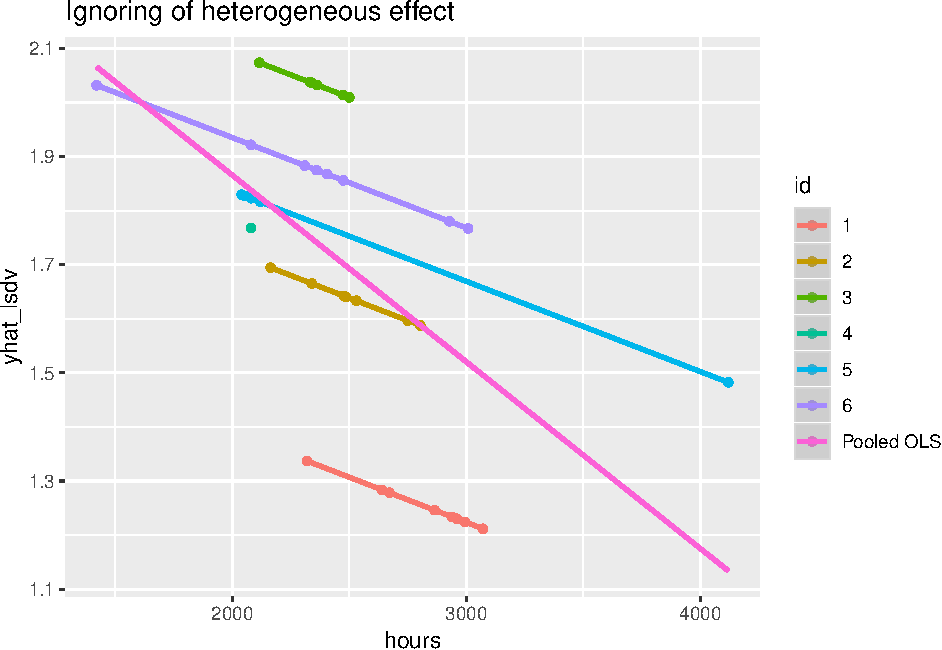
\includegraphics{09-paneldata_files/figure-latex/ignoring hetero-1.pdf}

Теперь то же самое в Stata

Для начала подгрузим данные и посмотрим на них. Сперва визуализируем
малый датасет.

\begin{verbatim}
use lwage_panel_small
summarize
\end{verbatim}

\begin{verbatim}
    Variable |       Obs        Mean    
> Std. Dev.       Min        Max
-------------+--------------------------
> ------------------------------
          nr |        48    364.6667    
> 390.3276         13        910
        year |        48      1983.5    
> 2.315535       1980       1987
       black |        48          .5    
> .5052912          0          1
       exper |        48    5.833333    
> 2.636353          1         11
        hisp |        48           0    
>        0          0          0
-------------+--------------------------
> ------------------------------
       hours |        48    2407.875    
> 425.1116       1420       4120
     married |        48       .1875    
> .3944428          0          1
        educ |        48          13    
>  .825137         12         14
       union |        48        .125    
> .3342187          0          1
       lwage |        48    1.724878    
> .4719456  -.7202626   2.873161
-------------+--------------------------
> ------------------------------
     expersq |        48    40.83333    
>   31.933          1        121
  occupation |        48    4.083333    
> 2.359529          1          9
          id |        48         3.5    
> 1.725898          1          6
\end{verbatim}

\begin{verbatim}
xtset id year
xtline hours, overlay
clear
\end{verbatim}

\begin{verbatim}
       panel variable:  id (strongly bal
> anced)
        time variable:  year, 1980 to 19
> 87
                delta:  1 unit
\end{verbatim}

\begin{verbatim}
use lwage_panel_large
xtset id year
summarize
\end{verbatim}

\begin{verbatim}
       panel variable:  id (strongly bal
> anced)
        time variable:  year, 1980 to 19
> 87
                delta:  1 unit

    Variable |       Obs        Mean    
> Std. Dev.       Min        Max
-------------+--------------------------
> ------------------------------
          nr |      4360    5262.059    
>  3496.15         13      12548
        year |      4360      1983.5    
> 2.291551       1980       1987
       black |      4360    .1155963    
> .3197769          0          1
       exper |      4360    6.514679    
> 2.825873          0         18
        hisp |      4360    .1559633    
> .3628622          0          1
-------------+--------------------------
> ------------------------------
       hours |      4360    2191.257    
> 566.3523        120       4992
     married |      4360    .4389908    
> .4963208          0          1
        educ |      4360    11.76697    
> 1.746181          3         16
       union |      4360    .2440367    
> .4295639          0          1
       lwage |      4360    1.649147    
> .5326094  -3.579079    4.05186
-------------+--------------------------
> ------------------------------
     expersq |      4360    50.42477    
> 40.78199          0        324
  occupation |      4360    4.988532    
> 2.319978          1          9
          id |      4360         273    
> 157.3457          1        545
\end{verbatim}

Визуализируем данные. Если необходимо разнести линии на разные графики,
следует убрать прараметр `overlay'.

Сгенерируем новую переменную и оценим модель с фиксированными эффектами.
Последний аргумент произведёт оценку стандартных ошибок переменных в
форме Хубера/Уайта

\begin{verbatim}

xtreg lwage hours, fe vce(robust)
\end{verbatim}

\begin{verbatim}
Fixed-effects (within) regression       
>         Number of obs      =      4360
Group variable: id                      
>         Number of groups   =       545

R-sq:  within  = 0.0000                 
>         Obs per group: min =         8
       between = 0.0004                 
>                        avg =       8.0
       overall = 0.0001                 
>                        max =         8

                                        
>         F(1,544)           =      0.00
corr(u_i, Xb)  = -0.0144                
>         Prob > F           =    0.9822

                                   (Std.
>  Err. adjusted for 545 clusters in id)
----------------------------------------
> --------------------------------------
             |               Robust
       lwage |      Coef.   Std. Err.   
>    t                                  
>         P>|t|                         
>                   [95% Con            
>                           f. Interval]
-------------+--------------------------
> --------------------------------------
       hours |  -5.59e-07   .0000251    
> -0.02                                 
>         0.982                         
>                  -.0000498            
>                               .0000487
       _cons |   1.650371   .0549505    
> 30.03                                 
>         0.000                         
>                    1.54243            
>                               1.758312
-------------+--------------------------
> --------------------------------------
     sigma_u |  .39075125
     sigma_e |  .38728237
         rho |  .50445844   (fraction of
>  variance due to u_i)
----------------------------------------
> --------------------------------------
\end{verbatim}

Сделаем то же самое для модели со случайными эффектами.

\begin{verbatim}
xtreg lwage hours, re vce(robust)
\end{verbatim}

\begin{verbatim}
Random-effects GLS regression           
>         Number of obs      =      4360
Group variable: id                      
>         Number of groups   =       545

R-sq:  within  = 0.0000                 
>         Obs per group: min =         8
       between = 0.0004                 
>                        avg =       8.0
       overall = 0.0001                 
>                        max =         8

                                        
>         Wald chi2(1)       =      0.00
corr(u_i, X)   = 0 (assumed)            
>         Prob > chi2        =    0.9510

                                   (Std.
>  Err. adjusted for 545 clusters in id)
----------------------------------------
> --------------------------------------
             |               Robust
       lwage |      Coef.   Std. Err.   
>    z                                  
>         P>|z|                         
>                   [95% Con            
>                           f. Interval]
-------------+--------------------------
> --------------------------------------
       hours |   1.46e-06   .0000238    
>  0.06                                 
>         0.951                         
>                  -.0000451            
>                               .0000481
       _cons |   1.645945   .0549594    
> 29.95                                 
>         0.000                         
>                   1.538227            
>                               1.753664
-------------+--------------------------
> --------------------------------------
     sigma_u |  .36626431
     sigma_e |  .38728237
         rho |   .4721295   (fraction of
>  variance due to u_i)
----------------------------------------
> --------------------------------------
\end{verbatim}

Тест Хаусмана.

\begin{verbatim}
xtreg lwage hours, re
estimates store b_re
xtreg lwage hours, fe
estimates store b_fe
hausman b_fe b_re, sigmamore
\end{verbatim}

\begin{verbatim}
Random-effects GLS regression           
>         Number of obs      =      4360
Group variable: id                      
>         Number of groups   =       545

R-sq:  within  = 0.0000                 
>         Obs per group: min =         8
       between = 0.0004                 
>                        avg =       8.0
       overall = 0.0001                 
>                        max =         8

                                        
>         Wald chi2(1)       =      0.01
corr(u_i, X)   = 0 (assumed)            
>         Prob > chi2        =    0.9128

----------------------------------------
> --------------------------------------
       lwage |      Coef.   Std. Err.   
>    z                                  
>         P>|z|                         
>                   [95% Con            
>                           f. Interval]
-------------+--------------------------
> --------------------------------------
       hours |   1.46e-06   .0000133    
>  0.11                                 
>         0.913                         
>                  -.0000247            
>                               .0000276
       _cons |   1.645945   .0337055    
> 48.83                                 
>         0.000                         
>                   1.579884            
>                               1.712007
-------------+--------------------------
> --------------------------------------
     sigma_u |  .36626431
     sigma_e |  .38728237
         rho |   .4721295   (fraction of
>  variance due to u_i)
----------------------------------------
> --------------------------------------



Fixed-effects (within) regression       
>         Number of obs      =      4360
Group variable: id                      
>         Number of groups   =       545

R-sq:  within  = 0.0000                 
>         Obs per group: min =         8
       between = 0.0004                 
>                        avg =       8.0
       overall = 0.0001                 
>                        max =         8

                                        
>         F(1,3814)          =      0.00
corr(u_i, Xb)  = -0.0144                
>         Prob > F           =    0.9682

----------------------------------------
> --------------------------------------
       lwage |      Coef.   Std. Err.   
>    t                                  
>         P>|t|                         
>                   [95% Con            
>                           f. Interval]
-------------+--------------------------
> --------------------------------------
       hours |  -5.59e-07    .000014    
> -0.04                                 
>         0.968                         
>                   -.000028            
>                               .0000269
       _cons |   1.650371   .0312611    
> 52.79                                 
>         0.000                         
>                   1.589081            
>                               1.711661
-------------+--------------------------
> --------------------------------------
     sigma_u |  .39075125
     sigma_e |  .38728237
         rho |  .50445844   (fraction of
>  variance due to u_i)
----------------------------------------
> --------------------------------------
F test that all u_i=0:     F(544, 3814) 
> =     8.14           Prob > F = 0.0000

                 ---- Coefficients ----
             |      (b)          (B)    
>         (b-B)                         
>                   sqrt(diag(V_b-V_B))
             |      b_fe         b_re   
>                                       
>      Difference                       
>                          S.E.
-------------+--------------------------
> --------------------------------------
       hours |   -5.59e-07     1.46e-06 
>       -2.02e-06                       
>                        4.26e-06
----------------------------------------
> --------------------------------------
                           b = consisten
> t under Ho and Ha; obtained from xtreg
            B = inconsistent under Ha, e
> fficient under Ho; obtained from xtreg

    Test:  Ho:  difference in coefficien
> ts not systematic

                  chi2(1) = (b-B)'[(V_b-
> V_B)^(-1)](b-B)
                          =        0.22
                Prob>chi2 =      0.6354
\end{verbatim}


\end{document}
